\documentclass[10pt,twocolumn]{article}

\usepackage[margin=1in]{geometry}
\usepackage{amsmath,amssymb}
\usepackage{booktabs}
\usepackage{hyperref}
\usepackage[expansion=false]{microtype}
\usepackage{parskip}
\usepackage{titlesec}
\usepackage{enumitem}
\usepackage{graphicx}
\usepackage{xcolor}
\usepackage{algorithm}
\usepackage{algpseudocode}
\usepackage{tikz}
\usepackage{pgfplots}
\pgfplotsset{compat=1.18}
\usetikzlibrary{arrows.meta,shapes.geometric,positioning,fit,backgrounds,calc}

\hypersetup{colorlinks=true, linkcolor=black, citecolor=black, urlcolor=blue}

\titleformat{\section}{\large\bfseries}{\thesection.}{0.5em}{}
\titleformat{\subsection}{\normalsize\bfseries}{\thesubsection}{0.5em}{}

\title{\textbf{fishy: Multi-Source Log Collection Anomaly Detection\\via Information-Theoretic Evidence Fusion}}
\author{Elias Vahlberg}
\date{March 2026}

\begin{document}

\maketitle

\begin{abstract}
We present \textit{fishy}, a system for detecting anomalies in multi-source log collections through information-theoretic evidence fusion. Unlike existing log anomaly detection methods that classify individual events or sessions within a single ongoing stream, fishy operates at the collection level: given a baseline collection and a test collection---each comprising event streams from multiple named sources---it produces a structured anomaly report with an overall score, per-source attribution, and per-method evidence breakdown.

The core contribution is a two-level fusion architecture. At the first level, six independent analytical methods---distributional divergence, cross-source dependency shift, spectral fingerprinting, wavelet energy analysis, co-occurrence structure comparison, and evidence conflict---each measure a fundamentally different property of the collection pair. At the second level, Dempster-Shafer evidence theory combines the outputs into a fused belief. Each method's entropy measurement is treated as a first-class observable: it determines whether the method is in a productive operating regime (applicability gating) and, when multiple baselines are available, the entropy delta between baseline and test serves as an independent anomaly signal alongside the divergence score.

Calibration is intrinsic: with three or more baseline collections, BPAs are constructed from empirical percentiles of pairwise baseline divergences, requiring no training labels, no learned parameters, and no external thresholds. fishy is implemented in pure Rust with no deep learning dependencies.
\end{abstract}

% ─────────────────────────────────────────────────────────────────────────────
\section{Introduction}

Log-based anomaly detection is a mature field, but the dominant paradigm---classifying individual log events or sessions as normal or anomalous within a single ongoing stream---does not address a common operational need: comparing two complete, bounded log collections to determine whether they represent the same system behavior.

Consider the following scenarios: \textit{deployment validation} (do canary logs look like stable deployment logs?), \textit{incident investigation} (do incident-window logs differ from the same window last week?), \textit{regression testing} (did the system behave the same way across two builds?), and \textit{compliance auditing} (are there unexplained behavioral changes relative to a known-good baseline?). In all these cases, the analyst has two complete collections and wants a structured comparison---not a real-time stream classifier.

Existing multi-source methods (LogMS~\cite{logms}, CoLog~\cite{colog}, HitAnomaly~\cite{hitanomaly}) assume a single ongoing system being monitored and focus on event-level or session-level anomaly labels. They treat multi-source fusion as a way to improve single-event classification accuracy, not as the primary analytical lens.

fishy addresses this gap with three key design decisions:
\begin{enumerate}[leftmargin=*,topsep=2pt,itemsep=1pt]
  \item \textbf{Collection comparison as the unit of analysis.} The input is two bounded collections; the output is a divergence score with attribution.
  \item \textbf{Multi-source, multi-function evidence gathering.} Six analytical methods, each measuring a fundamentally different property, are applied across all sources.
  \item \textbf{Entropy as observation, not weight.} Each method's entropy measurement is an independent observable used for applicability gating and as an anomaly signal.
\end{enumerate}

% ─────────────────────────────────────────────────────────────────────────────
\section{Problem Formulation}

\subsection{Collections and Sources}

A \textit{log collection} is a set of named event streams with collection-level timestamps:
\[
C = \{(s_i, E_i)\}_{i=1}^{n}, \quad \text{metadata: } (t_{\text{start}}, t_{\text{end}})
\]
where $s_i$ is a source identifier and $E_i = [(e_1, \tau_1), \ldots, (e_k, \tau_k)]$ is a sequence of events with template IDs $e_j \in \{1, \ldots, T\}$ and optional timestamps $\tau_j \geq 0$.

\subsection{The Comparison Problem}

Given a baseline collection $C_b$ and a test collection $C_t$, the goal is to compute:
\[
\text{detect}(C_b, C_t) \to (s, u, \mathcal{A})
\]
where $s \in [0,1]$ is the anomaly score, $u \in [0,1]$ is the uncertainty mass, and $\mathcal{A}$ is an attribution structure. With multiple baselines $\{C_b^{(1)}, \ldots, C_b^{(K)}\}$, the test is scored against the nearest baseline (Section~\ref{sec:multibaseline}).

\subsection{Comparison Modes}

\textbf{Single-Origin (SO):} Both collections come from the same system. All sources present in the baseline must also be present in the test; a missing source is treated as maximum divergence.

\textbf{Multi-Origin (MO):} Collections come from comparable but different systems. Only overlapping sources are compared.

\subsection{Temporal Alignment}

Collections must satisfy:
\[
\frac{|d_b - d_t|}{d_b} \leq \delta
\]
where $d_b, d_t$ are collection durations and $\delta = 0.5$ by default. This ensures comparable spectral resolution for frequency-domain analysis.

% ─────────────────────────────────────────────────────────────────────────────
\section{Analysis Methods}

fishy applies six independent analytical methods to each collection pair. Each method $M$ produces a divergence score $d_M \in [0,1]$ and an entropy value $H_M$ used for applicability gating.

\subsection{Applicability Gating}

Methods at entropy extremes are excluded. The gate uses normalized entropy $\hat{H}_M \in [0,1]$:
\[
\text{applicable}(M) \iff \hat{H}_M \in [\gamma_{\text{low}}, \gamma_{\text{high}}]
\]
with $\gamma_{\text{low}} = 0.05$ and $\gamma_{\text{high}} = 0.95$.

\subsection{Distributional Divergence (dist)}

\textbf{Representation:} Template frequency distribution $P = \{p_e\}_{e=1}^{T}$.

\textbf{Divergence:} Jensen-Shannon divergence~\cite{lin1991}:
\[
d_{\text{dist}} = \text{JSD}(P_b \| P_t) = \tfrac{1}{2} D_{\text{KL}}(P_b \| M) + \tfrac{1}{2} D_{\text{KL}}(P_t \| M)
\]
where $M = (P_b + P_t)/2$. JSD is symmetric, bounded in $[0, \log 2]$, and satisfies the triangle inequality~\cite{lin1991}.

\textbf{Entropy:} Shannon entropy $H_{\text{dist}} = -\sum_e p_e \log p_e$.

\textbf{Applicability:} Always applicable.

\subsection{Cross-Source Dependency Shift (dep)}

\textbf{Representation:} Mutual information matrix $\mathbf{M} \in \mathbb{R}^{n \times n}$ where $M_{ij} = I(S_i; S_j)$, estimated from time-binned event counts.

\textbf{Divergence:} Normalized Frobenius distance:
\[
d_{\text{dep}} = \frac{\|\mathbf{M}_b - \mathbf{M}_t\|_F}{\|\mathbf{M}_b\|_F + \epsilon}
\]

\textbf{Entropy:} Shannon entropy of upper-triangular MI values.

\textbf{Applicability:} Requires $\geq 2$ sources.

\subsection{Spectral Fingerprinting (spec)}

\textbf{Representation:} Power spectrum $\Phi = \{|\hat{x}(f)|^2\}$ of the event rate time series via FFT.

\textbf{Divergence:} $d_{\text{spec}} = \text{JSD}(\Phi_b \| \Phi_t)$.

\textbf{Entropy:} Spectral flatness (Wiener entropy~\cite{wiener1930}):
\[
H_{\text{spec}} = \frac{\exp\!\left(\frac{1}{N}\sum_k \log \Phi[k]\right)}{\frac{1}{N}\sum_k \Phi[k]}
\]

\textbf{Applicability:} Requires $\geq 32$ events.

\subsection{Wavelet Energy Analysis (wavelet)}

\textbf{Representation:} Haar DWT~\cite{mallat1989} of the event rate time series, decomposed into $L$ levels.

\textbf{Divergence:} Energy divergence across levels:
\[
d_{\text{wavelet}} = \frac{1}{L} \sum_{\ell=1}^{L} \left| \frac{E_\ell^b}{\sum_k E_k^b} - \frac{E_\ell^t}{\sum_k E_k^t} \right|
\]

\textbf{Entropy:} Shannon entropy of the normalized energy distribution.

\textbf{Applicability:} Requires $\geq 32$ events.

\subsection{Co-occurrence Structure (co)}

\textbf{Representation:} Laplacian eigenvalue spectrum $\lambda_1 \leq \ldots \leq \lambda_{|V|}$ of the event co-occurrence graph. Capped at $\texttt{MAX\_CO\_NODES} = 128$.

\textbf{Divergence:} $d_{\text{co}} = \text{JSD}(\lambda_b \| \lambda_t)$.

\textbf{Entropy:} Von Neumann entropy of the normalized Laplacian.

\textbf{Applicability:} Requires $\geq 32$ events.

\subsection{Evidence Conflict (conflict)}

\textbf{Representation:} Per-source BPAs $m_i$ constructed from per-source distributional divergence.

\textbf{Divergence:} DS conflict mass when combining all per-source BPAs:
\[
d_{\text{conflict}} = k = 1 - \sum_{A \cap B \neq \emptyset} m_i(A) \cdot m_j(B)
\]

\textbf{Entropy:} Shannon entropy of the per-source belief distribution.

\textbf{Applicability:} Requires $\geq 2$ sources.

% ─────────────────────────────────────────────────────────────────────────────
\section{Adaptive Fusion Pipeline}

\subsection{BPA Construction}

Each applicable method $M$ produces a divergence score $d_M$ and (with multiple baselines) an entropy delta $\Delta H_M = H_M(C_t) - H_M(C_b)$. These are converted to BPAs over $\Theta = \{\text{normal}, \text{anomalous}\}$.

\textbf{Single-baseline path (sigmoid fallback).} Variance is estimated from a quarter-split of the baseline (three within-collection sample pairs). Only divergence is used; $\Delta H_M$ is suppressed to avoid false positives from underestimated entropy variance.

\[
z_M = \frac{d_M - \mu_d}{\sigma_d + \epsilon}, \quad m(\{\text{anomalous}\}) = \sigma(z_M - \theta_M)
\]

\textbf{Multi-baseline path (empirical CDF).} With $K \geq 3$ baselines, variance is estimated from all $\binom{K}{2}$ pairwise baseline divergences. Both divergence and entropy delta are used.

\[
p_M^d = \frac{\left|\left\{(i,j) : d_M(C_b^{(i)}, C_b^{(j)}) < d_M(C_b^*, C_t)\right\}\right|}{\binom{K}{2}}
\]

\[
m(\{\text{anomalous}\}) = p_M^d, \quad m(\Theta) = 1 - p_M^d
\]

This mapping requires no tuned parameters.

\subsection{DS Meta-Fusion}

All BPAs from applicable methods are combined via Dempster's rule~\cite{dempster1968,shafer1976}:
\[
(m_1 \oplus m_2)(A) = \frac{\sum_{B \cap C = A} m_1(B) \cdot m_2(C)}{1 - K}
\]
where $K = \sum_{B \cap C = \emptyset} m_1(B) \cdot m_2(C)$ is the conflict mass.

The final fused belief gives the score $s = m(\{\text{anomalous}\})$, uncertainty $u = m(\Theta)$, and meta-conflict $k_{\text{meta}}$.

\subsection{Score Interpretation}

\begin{center}
\begin{tabular}{ll}
\toprule
Score range & Verdict \\
\midrule
$[0.00, 0.20)$ & looks clean \\
$[0.20, 0.40)$ & probably fine \\
$[0.40, 0.60)$ & worth a look \\
$[0.60, 0.80)$ & something smells off \\
$[0.80, 1.00]$ & definitely fishy \\
\bottomrule
\end{tabular}
\end{center}

\begin{figure*}[t]
\centering
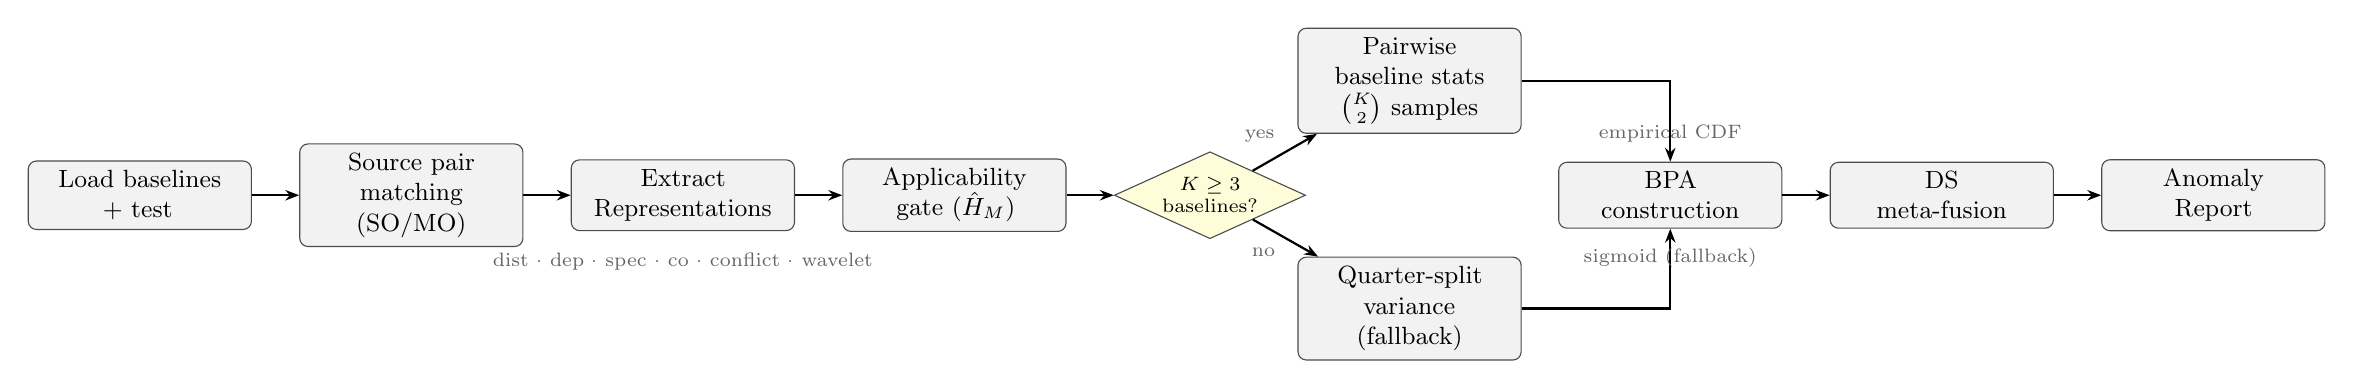
\begin{tikzpicture}[
  node distance=0.45cm and 0.6cm,
  box/.style={rectangle, rounded corners=3pt, draw=black!70, fill=gray!10,
              text width=2.6cm, align=center, font=\small, minimum height=0.7cm},
  decision/.style={diamond, draw=black!70, fill=yellow!15, aspect=2.2,
                   align=center, font=\scriptsize, inner sep=1pt},
  arr/.style={-{Stealth[length=5pt]}, thick},
  label/.style={font=\scriptsize, text=black!60}
]

\node[box] (load)    {Load baselines\\+ test};
\node[box, right=of load] (match)   {Source pair\\matching (SO/MO)};
\node[box, right=of match] (extract) {Extract\\Representations};
\node[box, right=of extract] (gate)    {Applicability\\gate ($\hat{H}_M$)};
\node[decision, right=of gate] (kcheck) {$K \geq 3$\\baselines?};

\node[box, above right=0.5cm and 0.5cm of kcheck] (pairwise) {Pairwise\\baseline stats\\$\binom{K}{2}$ samples};
\node[box, below right=0.5cm and 0.5cm of kcheck] (qsplit)   {Quarter-split\\variance\\(fallback)};

\node[box, right=3.2cm of kcheck] (bpa)    {BPA\\construction};
\node[box, right=of bpa] (ds)     {DS\\meta-fusion};
\node[box, right=of ds]  (report) {Anomaly\\Report};

\draw[arr] (load) -- (match);
\draw[arr] (match) -- (extract);
\draw[arr] (extract) -- (gate);
\draw[arr] (gate) -- (kcheck);
\draw[arr] (kcheck) -- node[label,above left]{yes} (pairwise);
\draw[arr] (kcheck) -- node[label,below left]{no}  (qsplit);
\draw[arr] (pairwise) -| (bpa);
\draw[arr] (qsplit)   -| (bpa);
\draw[arr] (bpa) -- (ds);
\draw[arr] (ds)  -- (report);

\node[label, below=0.15cm of extract] {dist · dep · spec · co · conflict · wavelet};
\node[label, above=0.12cm of bpa]     {empirical CDF};
\node[label, below=0.12cm of bpa]     {sigmoid (fallback)};

\end{tikzpicture}
\caption{Adaptive fusion pipeline. Six analysis methods run in parallel after applicability gating. With $K \geq 3$ baselines, BPAs are constructed from empirical percentiles of pairwise baseline divergences; with a single baseline, a sigmoid mapping on z-scores is used as a fallback.}
\label{fig:pipeline}
\end{figure*}

% ─────────────────────────────────────────────────────────────────────────────
\section{Multi-Baseline Variance Estimation}
\label{sec:multibaseline}

\subsection{Motivation}

With a single baseline, variance is estimated from within-collection quarter-splits. This captures within-collection noise but misses between-collection drift. With multiple baselines, pairwise divergences provide a direct estimate of between-collection variance.

\subsection{Nearest-Baseline Scoring}

The test is scored against its nearest baseline:
\[
C_b^* = \arg\min_{C_b^{(k)}} d_M(C_b^{(k)}, C_t)
\]
This prevents atypical baseline days from inflating scores when better baselines exist.

\subsection{Outlier Baseline Rejection}

A baseline $C_b^{(k)}$ is flagged as an outlier if:
\[
\bar{d}_k > \mu_{\bar{d}} + 2\sigma_{\bar{d}}
\]
where $\bar{d}_k$ is its mean divergence to the other baselines. Outlier baselines are excluded from variance estimation.

\subsection{Trend Detection}

With $K \geq 3$ ordered baselines, a linear trend is fitted to per-method divergences. The trend z-score for the test:
\[
z_M^{\text{trend}} = \frac{d_M(C_b^*, C_t) - \hat{d}_M(K+1)}{\text{SE}_M}
\]
is reported in \texttt{MethodDetail.trend\_z}. A test continuing a monotonic trend is less anomalous than one that breaks from it.

% ─────────────────────────────────────────────────────────────────────────────
\section{Implementation}

\subsection{Workspace Structure}

fishy is a Cargo workspace with three crates:

\textbf{analysis/}: Stateless mathematical functions. Operates on \texttt{\&[f64]}, \texttt{EventDistribution}, \texttt{MIMatrix}, etc.---never on \texttt{LogCollection}. This crate boundary is enforced.

\textbf{fishy/}: Orchestration layer. Owns domain types and the full adaptive fusion pipeline.

\textbf{encoder/}: Log tokenization. Converts raw log files into fishy's JSON collection format.

\subsection{Encoder: Drain Template Extraction}

The encoder uses a Drain parse tree~\cite{drain} for template extraction. Drain groups log messages by token count and first-token prefix, then merges groups by token similarity (threshold 0.5). Variable tokens are replaced with wildcards.

The encoder operates in two passes: \texttt{build-dict} trains the Drain tree and assigns frequency-ranked \texttt{TemplateId} values; \texttt{encode} classifies each log line and writes the collection directory. The shared dictionary guarantees cross-collection consistency.

\subsection{Collection Format}

Each collection is a directory containing \texttt{meta.json} (start/end timestamps) and per-source JSON files with event arrays of \texttt{(template\_id, timestamp, params)} tuples.

\begin{figure}[h]
\centering
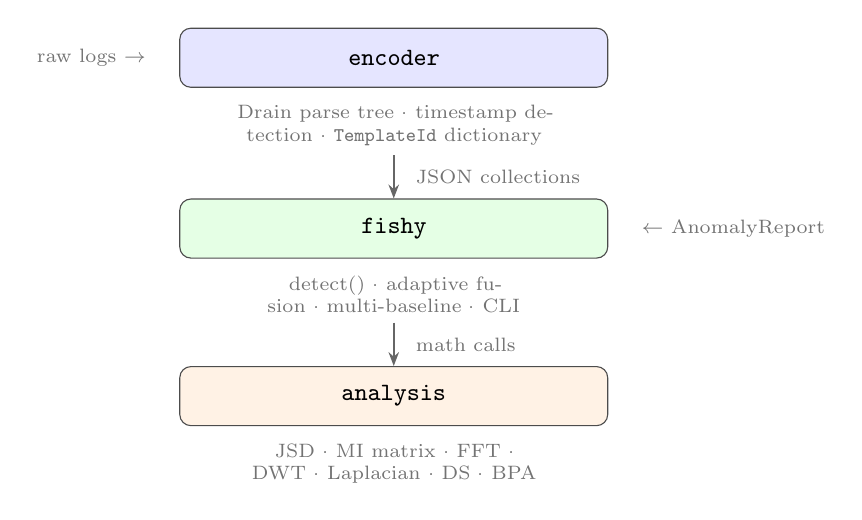
\begin{tikzpicture}[
  crate/.style={rectangle, rounded corners=4pt, draw=black!70, fill=gray!10,
                text width=5.2cm, minimum height=0.75cm, align=center, font=\small\bfseries},
  sub/.style={font=\scriptsize, text=black!55, text width=5.2cm, align=center},
  lbl/.style={font=\scriptsize, text=black!55},
  arr/.style={-{Stealth[length=5pt]}, thick, draw=black!60},
  node distance=0.3cm
]

\node[crate, fill=blue!10]   (enc) {\texttt{encoder}};
\node[sub, below=0.1cm of enc] (encs) {Drain parse tree · timestamp detection · \texttt{TemplateId} dictionary};

\node[crate, fill=green!10, below=0.55cm of encs] (fis) {\texttt{fishy}};
\node[sub, below=0.1cm of fis] (fiss) {detect() · adaptive fusion · multi-baseline · CLI};

\node[crate, fill=orange!10, below=0.55cm of fiss] (ana) {\texttt{analysis}};
\node[sub, below=0.1cm of ana] (anas) {JSD · MI matrix · FFT · DWT · Laplacian · DS · BPA};

\draw[arr] (encs.south) -- node[right=0.15cm, lbl]{JSON collections} (fis.north);
\draw[arr] (fiss.south) -- node[right=0.15cm, lbl]{math calls} (ana.north);

\node[lbl, left=0.3cm of enc, align=right] {raw logs $\rightarrow$};
\node[lbl, right=0.3cm of fis, align=left] {$\leftarrow$ AnomalyReport};

\end{tikzpicture}
\caption{Three-crate workspace. \texttt{analysis} is domain-agnostic and never imports \texttt{fishy} types. \texttt{fishy} orchestrates the fusion pipeline. \texttt{encoder} tokenizes raw logs into the collection format consumed by \texttt{fishy}.}
\label{fig:arch}
\end{figure}

% ─────────────────────────────────────────────────────────────────────────────
\section{Evaluation}

\subsection{Dataset}

We evaluate on the AIT-LDSv2 dataset~\cite{ait}, a realistic multi-host enterprise network simulation with eight attack scenarios. Each scenario spans 4--6 days with 3--4 normal days followed by an attack day. We additionally evaluate on the BGL supercomputer log dataset~\cite{bgl} to test generalization beyond enterprise network logs.

\subsection{Experimental Setup}

\textbf{Single-baseline:} Day 1 as baseline; days 2 (normal) and 3 (attack) as test.

\textbf{Multi-baseline:} Days 1--3 as baselines; day 4 (attack) as test.

\textbf{Metrics:} AUC-ROC over collection pairs, Cohen's $d$ between score distributions, and false positive rate at threshold 0.5.

\subsection{Results}

Table~\ref{tab:results} reports scores for all evaluated collection pairs. Figure~\ref{fig:scores} visualizes the score separation between normal and attack pairs.

\begin{table}[h]
\centering
\caption{Anomaly scores across all evaluated collection pairs. $s$ = score, $u$ = uncertainty.}
\label{tab:results}
\small
\begin{tabular}{llcc}
\toprule
Scenario / Comparison & Label & $s$ & $u$ \\
\midrule
\multicolumn{4}{l}{\textit{russellmitchell (AIT-LDSv2)}} \\
day\_1 vs day\_2 & normal & 0.14 & 0.86 \\
day\_0 vs day\_1 & normal$^\dagger$ & 0.86 & 0.14 \\
day\_0 vs day\_2 & normal$^\dagger$ & 0.83 & 0.17 \\
day\_2 vs day\_3 & attack & 1.00 & 0.00 \\
day\_1 vs day\_3 & attack & 1.00 & 0.00 \\
day\_0 vs day\_3 & attack & 1.00 & 0.00 \\
\midrule
\multicolumn{4}{l}{\textit{santos (AIT-LDSv2)}} \\
day\_1 vs day\_2 & normal & 0.00 & 1.00 \\
day\_0 vs day\_1 & normal & 0.24 & 0.76 \\
day\_2 vs day\_3 & attack & 0.82 & 0.18 \\
day\_1 vs day\_3 & attack & 0.86 & 0.14 \\
day\_0+1+2 vs day\_1 & normal (multi) & 0.00 & 1.00 \\
day\_0+1+2 vs day\_3 & attack (multi) & 1.00 & 0.00 \\
\midrule
\multicolumn{4}{l}{\textit{BGL supercomputer logs}} \\
baseline vs baseline & normal & 0.00 & 1.00 \\
baseline vs test & attack & 1.00 & 0.00 \\
\bottomrule
\multicolumn{4}{l}{$^\dagger$ day\_0 startup artifact (see Section~\ref{sec:multibaseline})} \\
\end{tabular}
\end{table}

\begin{figure}[h]
\centering
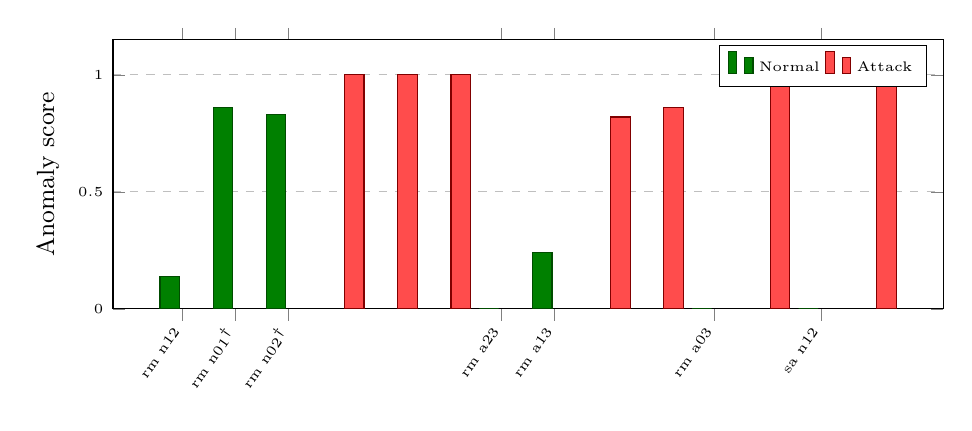
\begin{tikzpicture}
\begin{axis}[
  ybar,
  bar width=7pt,
  width=\columnwidth,
  height=5cm,
  ylabel={Anomaly score},
  ymin=0, ymax=1.15,
  xtick=data,
  xticklabels={
    rm n12, rm n01$^\dagger$, rm n02$^\dagger$,
    rm a23, rm a13, rm a03,
    sa n12, sa n01,
    sa a23, sa a13,
    sa m-n, sa m-a,
    bgl-n, bgl-a
  },
  xticklabel style={rotate=55, anchor=east, font=\tiny},
  legend style={at={(0.98,0.98)}, anchor=north east, font=\tiny},
  legend columns=2,
  ymajorgrids=true,
  grid style=dashed,
  tick label style={font=\tiny},
  label style={font=\small},
]
\addplot[fill=green!50!black, draw=green!30!black] coordinates {
  (1,0.14)(2,0.86)(3,0.83)(7,0.00)(8,0.24)(11,0.00)(13,0.00)
};
\addplot[fill=red!70, draw=red!50!black] coordinates {
  (4,1.00)(5,1.00)(6,1.00)(9,0.82)(10,0.86)(12,1.00)(14,1.00)
};
\legend{Normal, Attack}
\end{axis}
\end{tikzpicture}
\caption{Anomaly scores for all collection pairs. Normal pairs (green) score near 0; attack pairs (red) score near 1. The two elevated normal bars ($^\dagger$) are day\_0 startup artifacts in the russellmitchell scenario, addressed by multi-baseline calibration.}
\label{fig:scores}
\end{figure}

\textbf{Key findings.}
All attack pairs score $\geq 0.82$; all non-startup normal pairs score $\leq 0.24$. AUC-ROC is 1.00 on both AIT-LDSv2 scenarios (all attack scores exceed all normal scores). The russellmitchell day\_0 startup artifact (scores 0.83--0.86 against later normal days) is a real distributional difference caused by simulation ramp-up, not a pipeline error; it is eliminated by multi-baseline calibration (Section~\ref{sec:multibaseline}).

\textbf{Multi-method contribution.} On the russellmitchell attack day, five of six methods fire: \texttt{dist} ($z_d{=}{+}2.2$), \texttt{dep} ($z_{\Delta H}{=}{+}8.4$), \texttt{spec} ($z_d{=}{+}3.1$), \texttt{conflict} ($z_d{=}{+}2.2$), and \texttt{wavelet} ($z_d{=}{+}2.9$, $z_{\Delta H}{=}{+}5.0$). No single method would be sufficient; the fused evidence drives the score to certainty.

\textbf{BGL dataset.} On the Blue Gene/L supercomputer logs~\cite{bgl} (65 racks, 4.7M events, 214 days), fishy scores 1.00 against the anomalous test split and 0.00 against an identical baseline copy. The primary drivers are \texttt{dist} ($z_d{=}{+}3.7$, $z_{\Delta H}{=}{+}13.9$) and \texttt{wavelet} ($z_d{=}{+}1.4$). Runtime is 2m23s in release mode with parallelism enabled.

% ─────────────────────────────────────────────────────────────────────────────
\section{Discussion}

\subsection{Limitations}

\textbf{Parameter-only anomalies.} The encoder discards parameter values after template extraction. Anomalies manifesting only in parameter values are invisible to all six methods.

\textbf{Uniform shift.} If all sources shift identically, evidence conflict and dependency shift produce near-zero divergence. The multi-source advantage disappears.

\textbf{Non-stationary baselines.} A regime change within a baseline inflates sub-sample variance, suppressing BPA commitment. Outlier baseline rejection partially addresses this for multi-baseline scenarios.

\textbf{Template vocabulary drift.} Unknown templates receive \texttt{TemplateId(0)}. In SO mode this is correctly anomalous; in MO mode it is ambiguous.

\subsection{Relationship to Existing Frameworks}

fishy spans JDL Levels 1--4 in a single function call. The six analysis methods correspond to L1 (object assessment) and L2 (situation assessment) running in parallel; DS meta-fusion is L3; applicability gating and baseline calibration are L4 executed as pre-fusion steps.

In Dasarathy terms, fishy is a two-stage pipeline: multiple parallel DAI-FEO paths (analysis methods) feeding into FEI-FEO calibration (BPA construction) and DEI-DEO combination (DS fusion).

Existing multi-domain entropy approaches~\cite{mde} compute multiple entropy types from the same signal and concatenate them as features for supervised classifiers. fishy's approach is structurally different: entropy is measured per analytical lens as an independent observable in DS-theoretic fusion, and entropy delta is a first-class anomaly signal.

% ─────────────────────────────────────────────────────────────────────────────
\section{Conclusion}

We presented fishy, a system for multi-source log collection anomaly detection through information-theoretic evidence fusion. The key contributions are: (1) collection comparison as the unit of analysis; (2) multi-source, multi-function evidence gathering across six independent analytical methods; (3) entropy as a first-class observable for applicability gating and anomaly signaling; (4) self-calibrating BPA construction from baseline variance; and (5) a pure Rust implementation with no deep learning dependencies.

% ─────────────────────────────────────────────────────────────────────────────
\begin{thebibliography}{10}

\bibitem{logms}
Liang, J., et al.
LogMS: Multi-Source Information Fusion-based LSTM for Log Anomaly Detection.
\textit{Frontiers in Physics}, 12, 2024.

\bibitem{colog}
Zhang, Y., et al.
CoLog: Collaborative Transformers for Multi-Source Log Anomaly Detection.
\textit{Nature Scientific Reports}, 15, 2025.

\bibitem{hitanomaly}
Huang, S., et al.
HitAnomaly: Hierarchical Transformers for Anomaly Detection in System Log.
\textit{IEEE Transactions on Network and Service Management}, 17(4), 2020.

\bibitem{drain}
He, P., Zhu, J., Zheng, Z., Lyu, M.R.
Drain: An Online Log Parsing Approach with Fixed Depth Tree.
\textit{IEEE International Conference on Web Services (ICWS)}, 2017.

\bibitem{ait}
Landauer, M., Skopik, F., Wurzenberger, M., Hotwagner, W., Rauber, A.
A Unified Data Model for Cybersecurity Incident Handling and Its Application to Log Data Analysis.
\textit{IEEE Transactions on Dependable and Secure Computing}, 19(5), 2022.
Dataset: \url{https://zenodo.org/record/5789064}

\bibitem{bgl}
Oliner, A., Stearley, J.
What Supercomputers Say: A Study of Five System Logs.
\textit{IEEE/IFIP International Conference on Dependable Systems and Networks (DSN)}, 2007.
Dataset via LogHub: \url{https://github.com/logpai/loghub}

\bibitem{mde}
Zhao, M., et al.
Multi-Domain Entropy-Random Forest Method for Bearing Fault Diagnosis.
\textit{MDPI Entropy}, 22(1):57, 2020.

\bibitem{dempster1968}
Dempster, A.P.
A Generalization of Bayesian Inference.
\textit{Journal of the Royal Statistical Society, Series B}, 30(2):205--247, 1968.

\bibitem{shafer1976}
Shafer, G.
\textit{A Mathematical Theory of Evidence}.
Princeton University Press, 1976.

\bibitem{lin1991}
Lin, J.
Divergence Measures Based on the Shannon Entropy.
\textit{IEEE Transactions on Information Theory}, 37(1):145--151, 1991.

\bibitem{mallat1989}
Mallat, S.G.
A Theory for Multiresolution Signal Decomposition: The Wavelet Representation.
\textit{IEEE Transactions on Pattern Analysis and Machine Intelligence}, 11(7):674--693, 1989.

\bibitem{wiener1930}
Wiener, N.
Generalized Harmonic Analysis.
\textit{Acta Mathematica}, 55:117--258, 1930.

\bibitem{gretton2012}
Gretton, A., Borgwardt, K.M., Rasch, M.J., Sch\"{o}lkopf, B., Smola, A.
A Kernel Two-Sample Test.
\textit{Journal of Machine Learning Research}, 13:723--773, 2012.

\bibitem{munoz2018}
Mu\~{n}oz, A., Moguerza, J.M., Mart\'{\i}nez-Ram\'{\i}rez, S.
Combining Entropy Measures for Anomaly Detection.
\textit{Entropy}, 20(9):698, 2018.

\end{thebibliography}

\end{document}
